% !TEX root = main.tex

\section{Задание №1}
\section*{Условие} 
Дана последовательность \({X_1}\), . . . , \({X_n}\), . . . независимых дискретных случайных величин. Удовлетворяет ли эта последовательность закону больших чисел, если ряд распределения случайной величины \({X_n}\) имеет следующий вид?

\begin{figure}[h!]
	\begin{center}
		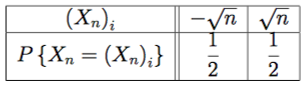
\includegraphics[width=180px]{table1}
	\end{center}
\end{figure}


\section*{Решение}
\begin{gather*} 
	MX_n = \sum_{i=1}^{n} X_iP_i = -\frac{\sqrt{n}}{2} + \frac{\sqrt{n}}{2} = 0
\end{gather*} 

\begin{gather*} 
	DX_n = \sum_{i=1}^{n} {X_i}^2P_i = \frac{n}{2} + \frac{n}{2} = n
\end{gather*}

-----
дальше надо переделать
% \(DX_n\) не зависит от n \(\Rightarrow\) ограниченно в совокупности
% (достаточное условие, что последовательность удовлетворяет ЗБЧ)

\section*{Ответ} 
Удовлетворяет ЗБЧ

\section{Задание №2}
\section*{Условие} 
С использованием метода моментов для выборки \(\vec{x_n}\) = (\({x_1}\), . . . , \({x_n}\)) найти точечные оценки параметров заданного закона распределения генеральной совокупности X.
\begin{figure}[h!]
	\begin{center}
		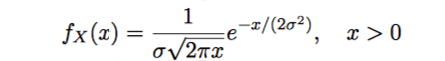
\includegraphics[width=250px]{table2}
	\end{center}
\end{figure}

\section*{Решение} 

\begin{gather*} 
\left.f_x(x) =
  \begin{cases}
    \frac{1}{\sigma\sqrt{2\pi x}}e^{\frac{-x}{2\sigma^2}}       & \quad \text{if } x >= 0\\
   	0  & \quad \text{else }\\
  \end{cases}
\right\}
\sim
\Gamma( \frac{1}{2\sigma^2},  \frac{1}{2} )
\end{gather*} 		

\noindentМетод моментов:
\begin{equation*} 
M_x = \frac{1/2}{1/(2\sigma^2)} = \sigma^2 = \bar{X_n}
\end{equation*}

\begin{equation*} 
	\widehat{\sigma} = \sqrt{\bar{X_n}}
\end{equation*}

\section*{Ответ} 
\begin{equation*} 
	\widehat{\sigma} = \sqrt{\bar{X_n}}
\end{equation*}

% \section{Задание №3}
% \section*{Условие} 
% С использованием метода максимального правдоподобия для выборки \(\vec{x_5}\) = (\({x_1}\), . . . , \({x_5}\)) найти точечные оценки параметров заданного закона распределения генеральной совокупности X.
% \begin{figure}[h!]
% 	\begin{center}
% 		
\includegraphics{table3}
% 	\end{center}
% \end{figure}
% \section*{Решение} 
% \section*{Ответ} 

\section{Задание №4}
\section*{Условие} 
После n = 11 независимых измерений случаийной величины X получены следующие значения: 

\begin{center}
9.9, 12.5, 10.3, 9.2, 6.0, 10.9, 10.3, 11.8, 11.6, 9.8, 14.0. 
\end{center}

\noindent Предполагая, что ошибки измерений распределены по нормальному закону, а систематические ошибки отсутствуют, определить: 
а) точечные оценки измеряемой величины и ее среднего квадратичного отклонения; 
б) вероятность того, что абсолютное значение ошибки при определении теоретического значения измеряемой величины меньше 2\% от \({X_n}\).
\section*{Решение} 

\begin{equation*} 
	\vec{X_n} = (9.9, 12.5, 10.3, 9.2, 6.0, 10.9, 10.3, 11.8, 11.6, 9.8, 14.0)
\end{equation*}
\begin{equation*} 
	\bar{X_n} = 10,57273
\end{equation*}
\begin{equation*} 
	S_n(\vec{X_n}) = 1,95685
\end{equation*}

\begin{enumerate}
	\item Метод моментов для X \(\sim\) N(m, \(\sigma\))
	\begin{align*} 
		\widehat{m_1} &= \bar{X_n} = \widehat{m} \\
		\widehat{m_2} &= S_n(\vec{X_n}) = \widehat{\sigma}
	\end{align*}

	\item P\{-0,02\(\bar{X_n}\) < m-\(\bar{X_n}\) < 0,02\(\bar{X_n}\)\} = ?
	Ищем центральную статистику для мат. ожидания при неизвестном \(\sigma\):
	\begin{equation*} 
		g(\vec{X_n}, m) = \frac{m-\bar{X_n}}{S(\vec{X_n})}\sqrt{n} = 
		\frac{m-\bar{X_n}}{S_n(\vec{X_n})}\sqrt{n-1}
		\sim
		S_1(n-1)
	\end{equation*}
	Преобразуем неравенство под знаком вероятности к этой статистике: \\

	\begin{equation*}
	-0,02\bar{X_n} < m-\bar{X_n} < 0,02\bar{X_n}
	\end{equation*}	

	\begin{equation*}
		\frac{-0,02\bar{X_n}}{S_n(\vec{X_n})}\sqrt{n-1}
		<
		g(\vec{X_n}, m)
		<
		\frac{0,02\bar{X_n}}{S_n(\vec{X_n})}\sqrt{n-1}
	\end{equation*}	

	\begin{equation*}
		\frac{-0,02 * 10,57273 * \sqrt{10} }{1,95685}
		<
		g(\vec{X_n}, m)
		<
		\frac{0,02 * 10,57273 * \sqrt{10} }{1,95685}
		=
		0,34171
	\end{equation*}

	Тогда: \\

	\begin{gather*}
	P\{-0,02\bar{X_n} < m-\bar{X_n} < 0,02\bar{X_n}\} = P\{-0,34171 < g(\vec{X_n}, m) < 0,34171\} = \\
	= \int^{0,34171}_{-0,34171} f_{s_1\atop10}(g)\,dg 
	= 2\int^{0,34171}_{0} f_{s_1\atop10}(g)\,dg = \\
	= 2(F_{s_1\atop10}(0,34171) - F_{s_1\atop10}(0)) 
	= 2(0,63 - 0,5)
	= 0,26
	\end{gather*}

\end{enumerate}

\section*{Ответ}
\begin{enumerate}
	\item
		\begin{align*} 
			\widehat{m_1} &= \bar{X_n} = \widehat{m} \\
			\widehat{m_2} &= S_n(\vec{X_n}) = \widehat{\sigma}
		\end{align*}		

	\item
		\begin{gather*}
			P\{-0,02\bar{X_n} < m-\bar{X_n} < 0,02\bar{X_n}\} = 0,26
		\end{gather*} 
\end{enumerate}



